\subsubsection{UC\theuccount-PR - Redmine invia segnalazione al Producer Redmine}
    \begin{figure}[H]
		\centering
		\includegraphics[width=0.5\textwidth]{img/casi_d'uso/UC\theuccount.png}\\
		\caption{UC1-PR - Redmine invia segnalazione al Producer Redmine}
	\end{figure}
\begin{itemize}
	\item \textbf{Codice}: UC\theuccount-PR.
	\item \textbf{Titolo}: Redmine invia segnalazione al Producer Redmine.
	\item \textbf{Attori primari}: Redmine.
	\item \textbf{Descrizione}: Redmine invia a \progetto\ una segnalazione.
	\item \textbf{Precondizione}: su Redmine viene eseguita un'operazione che scaturisce una
	segnalazione da inviare a \progetto.
	\item \textbf{Postcondizione}: il Producer Redmine riceve la segnalazione da Redmine.
	\item \textbf{Scenario principale}:
	\begin{enumerate}
		\item Viene eseguita un'operazione in Redmine da far scaturire l'invio di una segnalazione
		\item Redmine procede all'invio della segnalazione al Producer Redmine
        \item La segnalazione viene ricevuta dal Producer Redmine
	\end{enumerate}

\end{itemize}

\stepcounter{subuccount}

\subsubsection{UC\theuccount.\thesubuccount-PR - Redmine segnala apertura issue al Producer Redmine}
%    \begin{figure}[H]
%		\centering
%		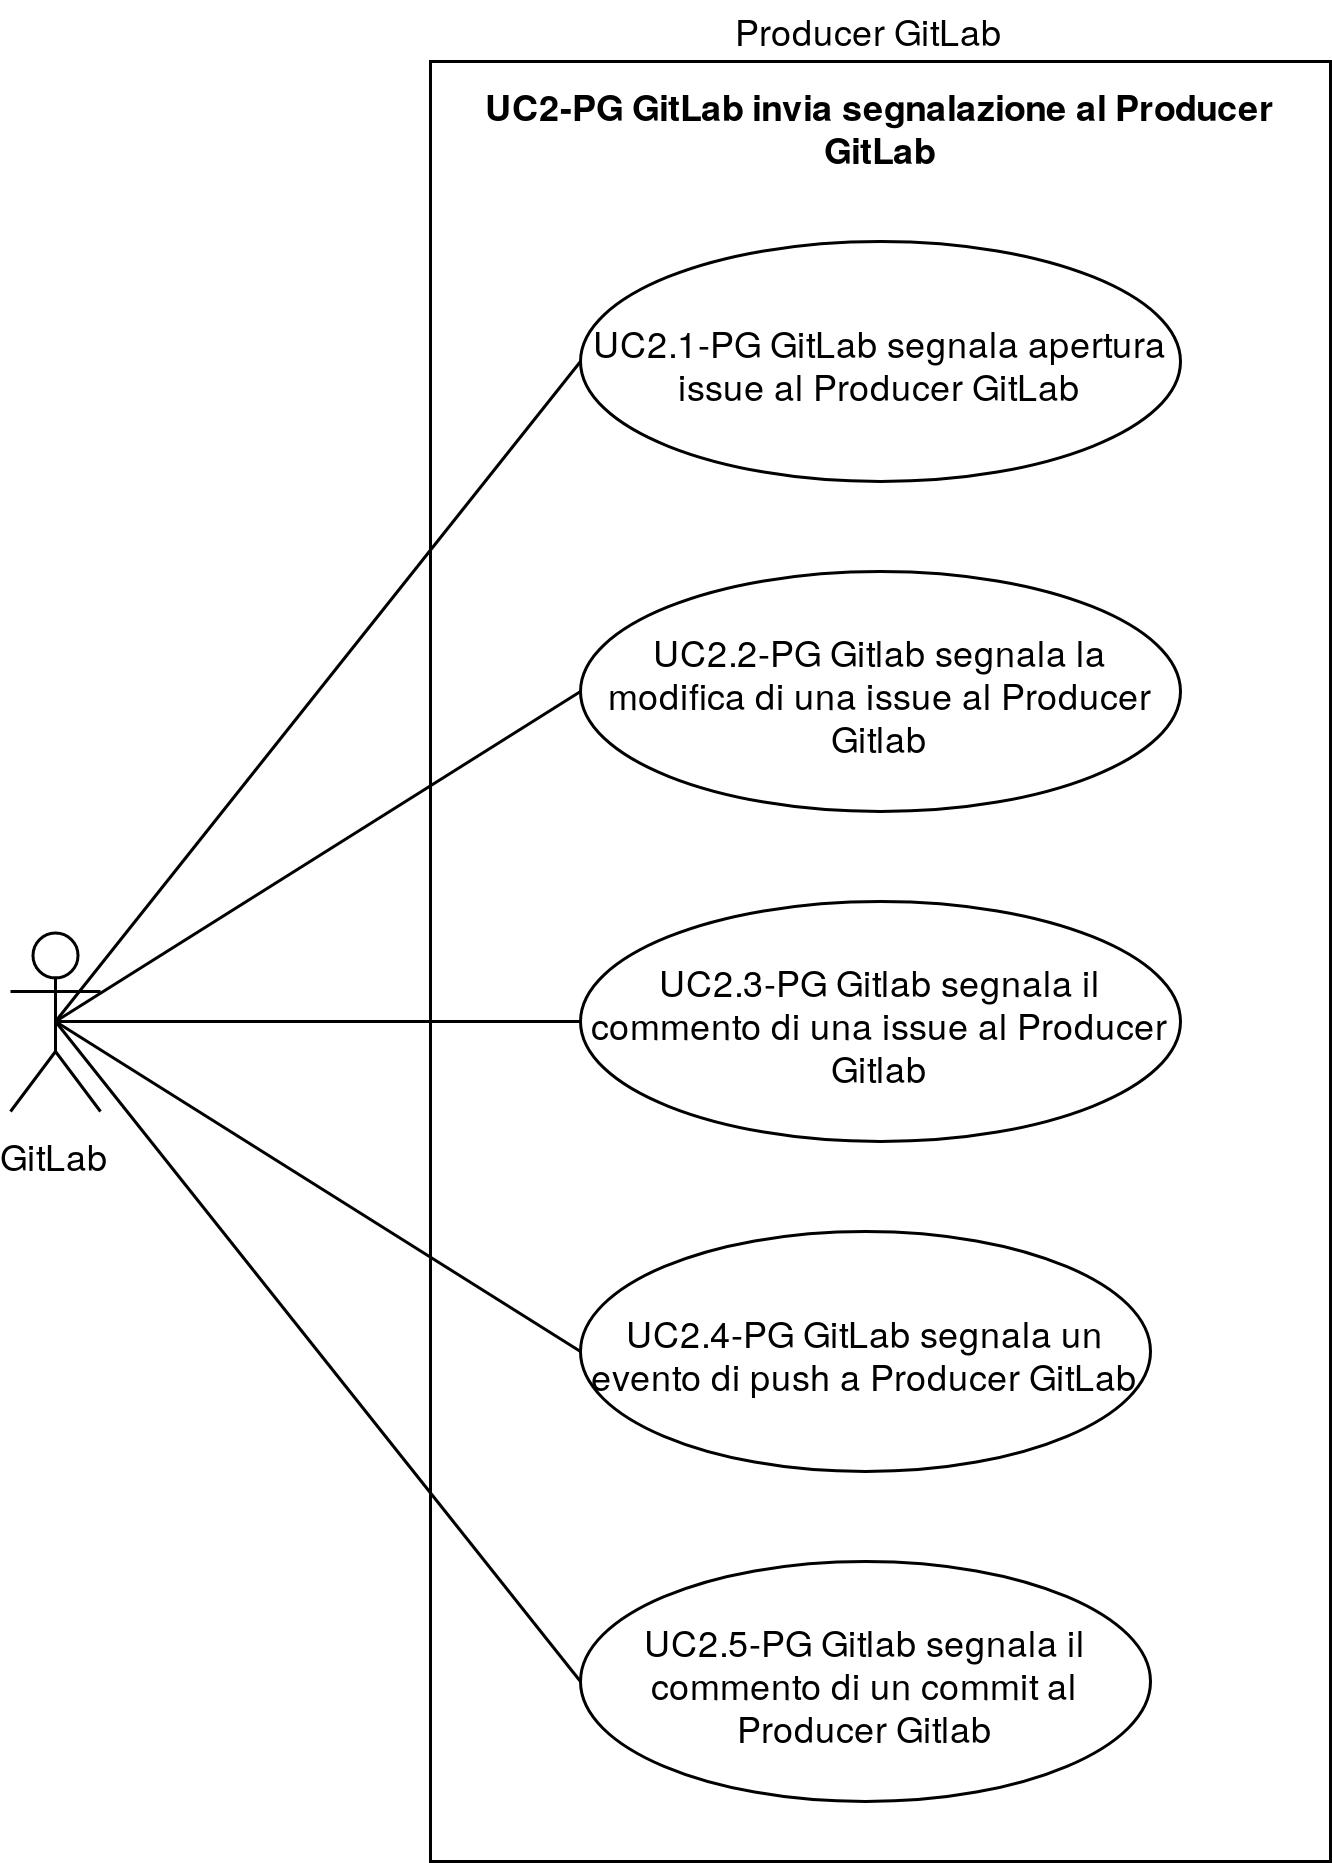
\includegraphics[width=0.5\textwidth]{img/casi_d'uso/UC2.png}\\
%		\caption{UC\theuccount-PR - Redmine segnala apertura issue al Producer Redmine}
%	\end{figure}
\begin{itemize}
	\item \textbf{Codice}: UC\theuccount.\thesubuccount-PR.
	\item \textbf{Titolo}: Redmine segnala apertura issue al Producer Redmine.
	\item \textbf{Attori primari}: Redmine.
	\item \textbf{Descrizione}: Redmine segnala a \progetto\ l'apertura di una nuova issue tramite webhook.

	L'apertura di una issue in un particolare progetto su Redmine contiene i seguenti campi di interesse:
	\begin{itemize}
		\item Status
		\item Tracker
		\item Subject
		\item Priority e opzionalmente:
		\begin{itemize}
			\item Description
			\item Assignee
		\end{itemize}
	\end{itemize}
	Il campo status conterrà sempre al suo interno ``opened''.
	\item \textbf{Precondizione}: Viene aperta una issue su Redmine da
	segnalare a \progetto.
	\item \textbf{Postcondizione}: il Producer Redmine riceve la segnalazione di apertura issue da Redmine.
	\item \textbf{Scenario principale}:
	\begin{enumerate}
		\item Viene aperta una nuova issue su Redmine compilando i campi indicati
		\item Redmine procede all'invio della segnalazione di issue al Producer Redmine
        \item Il Producer Redmine riceve la segnalazione di apertura issue
	\end{enumerate}

\end{itemize}

\stepcounter{subuccount}

\subsubsection{UC\theuccount.\thesubuccount-PR - Redmine segnala la modifica di una issue al Producer Redmine}
%	\begin{figure}[H]
%		\centering
%		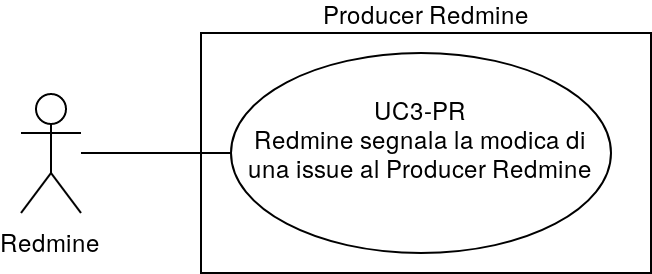
\includegraphics[width=0.5\textwidth]{img/casi_d'uso/UC3.png}\\
%		\caption{UC\theuccount-PR - Redmine segnala la modifica di una issue al Producer Redmine}
%	\end{figure}
\begin{itemize}
	\item \textbf{Codice}: UC\theuccount\thesubuccount-PR.
	\item \textbf{Titolo}: Redmine segnala la modifica di una issue al Producer Redmine.
	\item \textbf{Attori primari}: Redmine.
	\item \textbf{Descrizione}: quando una issue viene modificata, l'invio di tale segnalazione
	avviene da parte di Redmine tramite webhook.
	I campi di interesse sono gli stessi dell'apertura di una issue, con la differenza che necessariamente il campo status contiene ora ``updated''.
	\item \textbf{Precondizione}: Viene modificata una issue già aperta su un
	progetto di Redmine da segnalare a \progetto.
	\item \textbf{Postcondizione}: il Producer Redmine riceve la segnalazione di modifica issue da Redmine.
	\item \textbf{Scenario principale}:
	\begin{enumerate}
		\item Viene modificata una issue già esistente su Redmine
		\item Redmine procede all'invio della segnalazione di modifica issue al Producer Redmine
        \item Il Producer Redmine riceve la segnalazione di modifica issue
	\end{enumerate}

\end{itemize}

\stepcounter{subuccount}

\subsubsection{UC\theuccount.\thesubuccount-PR - Redmine segnala il commento di una issue al Producer Redmine}
%	\begin{figure}[H]
%		\centering
%		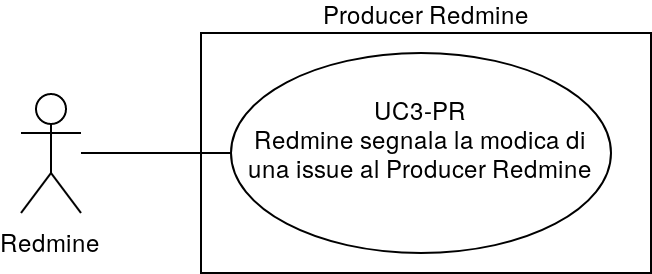
\includegraphics[width=0.5\textwidth]{img/casi_d'uso/UC3.png}\\
%		\caption{UC\theuccount-PR - Redmine segnala la modifica di una issue al Producer Redmine}
%	\end{figure}
\begin{itemize}
	\item \textbf{Codice}: UC\theuccount.\thesubuccount-PR.
	\item \textbf{Titolo}: Redmine segnala il commento di una issue al Producer Redmine.
	\item \textbf{Attori primari}: Redmine.
	\item \textbf{Descrizione}: quando una issue viene commentata, l'invio di tale segnalazione
	avviene da parte di Redmine tramite webhook.
	I campi di interesse sono gli stessi dell'apertura di una issue, con la differenza che necessariamente il campo status contiene ora ``updated''.
	\item \textbf{Precondizione}: Viene modificata una issue già aperta su un
	progetto di Redmine da segnalare a \progetto.
	\item \textbf{Postcondizione}: il Producer Redmine riceve la segnalazione del commento di una issue da Redmine.
	\item \textbf{Scenario principale}:
	\begin{enumerate}
		\item Viene modificata una issue già esistente su Redmine
		\item Redmine procede all'invio della segnalazione di modifica issue al Producer Redmine
	\end{enumerate}

\end{itemize}
